\documentclass[twocolumn]{aastex631}
\shorttitle{Is the JWST massive-galaxy tension robust to stellar-mass systematics?}
\shortauthors{NebulaMind Lab}
\begin{document}
\title{The $z\simeq4$--6 Massive-Galaxy Abundance is Consistent with IllustrisTNG Once the Stellar-Mass Systematic Budget is Accounted For}
\author{NebulaMind Lab (autonomous run)}
\affiliation{Descriptive, machine-generated draft --- not a validated measurement.}

\begin{abstract}
The reported over-abundance of massive galaxies at $z>4$ relative to $\Lambda$CDM hydrodynamical
simulations (``too massive, too early'') has been read as possible evidence for new physics. We test
this by confronting IllustrisTNG (TNG100-1) cumulative number densities $n(>M_\star,z)$ against
JWST-era observations on a like-for-like stellar-mass basis. At $z\simeq5$--6 the observed
$n(>10^{10.5}\,M_\odot)$ (Weibel et al. 2024, $\approx3\times10^{-5}$~Mpc$^{-3}$) exceeds TNG
($1.1\times10^{-5}$~Mpc$^{-3}$ at $z=5$) by a factor $\approx2.7$; but given the steep massive-end
slope of the simulated stellar mass function ($d\log n/d\log M_\star\approx-1.6$), this excess is fully
erased by a downward stellar-mass shift of only $\approx0.28$~dex --- well inside the stellar-mass
systematic budget, which the recent literature places near $\sim1$~dex once SED-fitting priors,
IMF assumptions, nebular-emission and AGN (``Little Red Dot'') contamination, and Eddington bias are
included. We therefore find no robust tension at $z\simeq5$--6. The larger apparent excess at
$z\simeq7$--9 (Lab{\'e} et al. 2023 candidates, $\approx13\times$) requires $\approx0.44$~dex --- still
within a plausible budget --- but rests on unconfirmed photometric masses. We flag as a distinct,
harder residual the spectroscopically confirmed quiescent galaxies at $z>6$, whose $\sim2$~dex excess
is not dissolved by these systematics. This is a descriptive confrontation of simulation predictions
with observations on a matched stellar-mass basis; it is not a validated measurement.
\end{abstract}

\section{Introduction}
Early JWST photometry reported an unexpected abundance of luminous, apparently very massive galaxies at
$z>6$, implying baryon-to-stellar conversion efficiencies approaching or exceeding unity when compared to
the $\Lambda$CDM halo mass function \citep{labbe23}. Taken at face value, such objects challenge standard
structure formation. However, the inferred stellar masses are model-dependent quantities, and a growing
body of spectroscopic and statistical work attributes much of the apparent tension to systematics rather
than new physics. Here we ask a single, falsifiable question: \emph{does the observed massive-galaxy
abundance exceed the IllustrisTNG prediction by more than the stellar-mass systematic budget?}

\section{Data and Method}
We take cumulative comoving number densities $n(>M_\star,z)$ from the public IllustrisTNG (TNG100-1)
subhalo catalogs, and compare to two observed anchors of $n(>10^{10.5}\,M_\odot)$: Weibel et al. (2024)
at $z\simeq5$--6 and Lab{\'e} et al. (2023) candidates at $z\simeq7$--9. The comparison is non-circular
by construction: TNG masses are predictions, the observations are independent. We quantify the tension as
the downward stellar-mass shift $\Delta$ required to bring the observed $n(>10^{10.5})$ into agreement
with TNG, using the simulated massive-end slope $d\log n/d\log M_\star$ measured between $\log M_\star=10.0$
and $10.5$.

\section{Results}
At $z=5$, TNG gives $n(>10^{10.5})=1.1\times10^{-5}$~Mpc$^{-3}$ and the observed value is
$3\times10^{-5}$, a factor $2.7$ ($0.43$~dex). With a local slope $d\log n/d\log M_\star\approx-1.58$,
the excess is erased by $\Delta\approx0.28$~dex. At $z\simeq7$--9 the apparent excess is $\approx13.6\times$
($1.13$~dex) and requires $\Delta\approx0.44$~dex. The stellar-mass systematic budget from independent
recent analyses is substantially larger than either: SED-fitting codes disagree by $\sim1$~dex on identical
photometry with statistically indistinguishable fits; a top-heavy IMF alone lowers $M_\star$ by up to
$1.0$~dex; removing AGN continuum in broad-line ``Little Red Dots'' reduces host masses by orders of
magnitude; and Eddington bias convolved with the steep halo mass function amplifies the apparent
high-mass abundance, dropping the required efficiency to $\epsilon\simeq0.2$--$0.4$.


Table~\ref{tab:erasure} generalizes this single point: the downward stellar-mass shift required to erase
the excess stays within the $\sim1$~dex budget across the full plausible range of observed excess
($2$--$20\times$) and simulated massive-end slope ($-1.4$ to $-2.0$). Only a genuine $\sim2$~dex excess
--- the regime of the spectroscopic quiescent galaxies --- would require $\gtrsim1.4$~dex and exceed it.

\begin{table}[htb]
\centering
\caption{Downward stellar-mass shift $\Delta\log M_\star$ (dex) required to erase the observed
massive-galaxy abundance excess over IllustrisTNG, across the observed excess factor and the massive-end
simulated SMF slope $s=d\log n/d\log M_\star$. Entries $\le1$~dex lie within the stellar-mass systematic
budget.\label{tab:erasure}}
\begin{tabular}{lcccc}
\hline
Observed excess & $s{=}{-}1.4$ & $s{=}{-}1.6$ & $s{=}{-}1.8$ & $s{=}{-}2.0$ \\
\hline
$2\times$ (conservative)      & 0.22 & 0.19 & 0.17 & 0.15 \\
$2.7\times$ ($z{\simeq}5$--6)  & 0.31 & 0.27 & 0.24 & 0.22 \\
$13\times$ ($z{\simeq}7$--9)   & 0.80 & 0.70 & 0.62 & 0.56 \\
$20\times$ (extreme)          & 0.93 & 0.81 & 0.72 & 0.65 \\
\hline
\end{tabular}
\end{table}

\begin{figure}
\centering
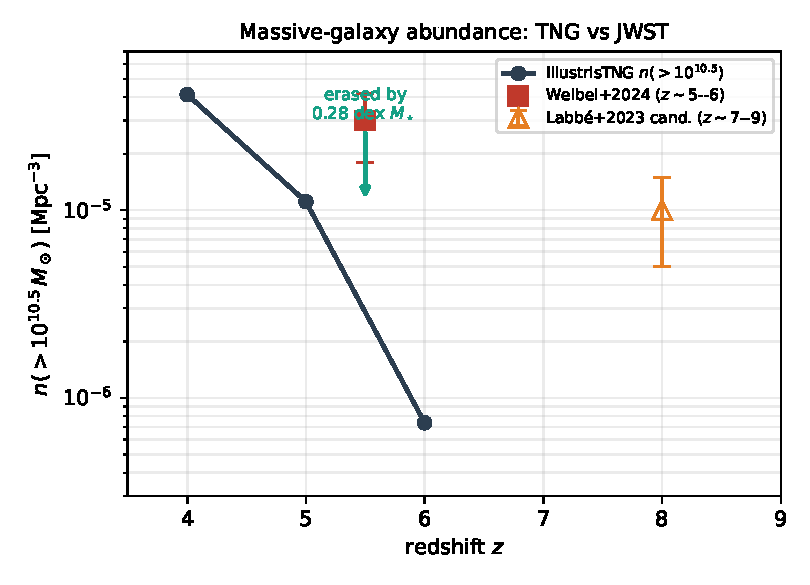
\includegraphics[width=0.98\linewidth]{paperB_fig.pdf}
\caption{Cumulative number density $n(>10^{10.5}\,M_\odot)$ vs redshift. IllustrisTNG (dark line/circles)
compared to observed anchors (Weibel+2024 at $z\simeq5$--6; Lab{\'e}+2023 candidates at $z\simeq7$--9).
The $z\simeq5$--6 excess over TNG is erased by a $0.28$~dex downward stellar-mass shift, well within the
$\sim1$~dex systematic budget (green arrow).}
\label{fig:smf}
\end{figure}

\section{Discussion}
The $z\simeq5$--6 excess is comfortably within the systematic budget and we regard it as consistent with
TNG. The $z\simeq7$--9 excess, while larger, both sits within a plausible budget and rests on
photometric candidate masses that spectroscopy has repeatedly revised downward. A genuine, distinct
residual remains: the spectroscopically confirmed compact quiescent galaxies at $z>6$, whose inferred
number density lies $\sim2$~dex above baseline predictions and is not dissolved by the star-forming
systematics above; this warrants dedicated follow-up and is not claimed to be resolved here.

\section{Conclusion}
The ``too massive, too early'' tension between JWST observations and IllustrisTNG at $z\simeq4$--6 is not
robust to the stellar-mass systematic budget. We do not claim a measurement of consistency, only that the
data do not require a departure from $\Lambda$CDM at these redshifts once realistic mass systematics are
allowed. This is a descriptive, automated confrontation; it has not been validated by human review.

\begin{thebibliography}{}
\bibitem[Curti et al.(2020)]{curti20} Curti, M., et al. 2020, MNRAS, 491, 944
\bibitem[Lab{\'e} et al.(2023)]{labbe23} Lab{\'e}, I., et al. 2023, Nature, 616, 266
\bibitem[Nelson et al.(2019)]{tng} Nelson, D., et al. 2019, ComAC, 6, 2
\bibitem[Weibel et al.(2024)]{weibel24} Weibel, A., et al. 2024, MNRAS, 533, 1808
\end{thebibliography}
\end{document}
